\documentclass[11pt,a4paper]{article}
\usepackage[utf8]{inputenc}
\usepackage[hmargin=2.0cm,vmargin=2.5cm,bindingoffset=0.5cm]{geometry}
\usepackage{amsfonts}
\usepackage{amsmath,amsthm,amssymb}
\usepackage{hyperref}
\usepackage{graphicx}
\usepackage{tikz}
\usepackage{mathtools}
\DeclarePairedDelimiter\ceil{\lceil}{\rceil}
\DeclarePairedDelimiter\floor{\lfloor}{\rfloor}
%\usepackage{float}
\usepackage{placeins}
\usepackage{diagbox}
\newtheorem{thm}{Theorem}
\usepackage{subcaption}
%\usepackage{subfigure}
\usepackage[english]{babel}
\author{Mohit}
\title{Counterdiabatic driving}
\begin{document}
\maketitle

\section{Goal}

The goal, as of now, is to distinguish between integrable and non-integrable many-body quantum system by studying their approximate gauge adiabatic potential\footnote{We expect results to be valid for classical system too. But for now, we would focus on quantum systems.}

 
Classically, on one hand, integrable systems have a lot of constants of motion, and as a result, they have a few independent degrees of freedom. On the other hand, non-integrable systems contain a large number of independent degrees of freedom. We expect a similar picture for quantum systems.

The central idea is to apply Eigenstate Thermalization Hypothesis (ETH) to operators of exact gauge potential in non-integrable quantum systems, and claim that its' norm scales exponentially in system 
size. Whereas for integrable systems, exact gauge potential are supposed to scale like a polynomial in system size.

\section{Introduction}
\subsection{Integrable and non-integrable systems}
What is an integrable quantum systems? To the best of my knowledge, the general definition of integrability for quantum systems has not been reached conclusively. Despite this, there are some models which are commonly agreed to be integrable and similarly, there are model which are called non-integrable in literature. For our purposes, we would use such models to get some intuition.

Let's list down a few properties of \textbf{integrable} quantum systems: 
\begin{itemize}
\item The many-body density matrix of those systems don't thermalize to Gibbs distribution. In fact, they thermalize to a generalized Gibbs distribution. (see \cite{rigol2007relaxation,cassidy2011generalized} for detail) 
\item They can be diagonalized using a transformation that is local in space\footnote{According to Dries, for 2D transverse quantum Ising model, Jordan Wigner transformation exists to diagonalize the Hamiltonian. However, it's still called a non-integrable model since then the transformation becomes non-local. I need to dig relevant paper for details}. Examples are non-interacting fermions, 1 D Ising model and 1D transverse field Ising model (TFIM).  These can be diagonalized using Bogoliubov, transfer matrix method and Jordan-Wigner transformation, respectively.
\item ETH doesn't apply to them 
\item Distribution of Energy level spacing follows Poisson distribution --energy level attraction.
\end{itemize}

We note here that many body localized (MBL) system is a new kind of integrable system. To understand its' similarity and difference from integrable system, I am quoting a paragraph from \cite{o2016explicit} : 

``In order to explain the basic phenomenology of MBL systems, including their failure to thermalise, a picture of Local Integrals of Motion (LIOMs) has been put forward. According to this picture, the basic mechanism of MBL is similar to integrable models: there emerges an extensive number of operators (“conserved charges”) $\tau_i$ , which commute amongst  themselves $[\tau_i , \tau_j ]=0$ as well as with the Hamiltonian $[H, \tau_i]=0$.

A special property of MBL systems is that $\tau_i$ have eigenvalues $\pm 1$, thus they resemble the bare spin-1/2 operators, and generically there are L such operators in a lattice system of size L. This means that any Hamiltonian eigenvector can be specified by the conserved quantum numbers corresponding to operators $\tau_i$. Because of this extensive number of emergent quantum numbers (that by definition do not change during unitary evolution), the thermalisation of the system is prevented as the MBL state retains the memory of its initial condition. \textbf{The difference between integrable models and MBL systems is in the form of individual $\tau_i$ : in the integrable case, each $\tau_i$. is an extended sum of local operators, while in the MBL case each $\tau_i$. is a single local operator, up to corrections that vanish exponentially with distance to the core.} The subleading (exponentially suppressed) corrections are important, as they cause the distinction between Anderson and MBL insulators. For example, the presence of tails in LIOMs is responsible for the dephasing dynamics and the spreading of entanglement in MBL systems, which does not occur in Anderson insulators"

In \cite{abanin2017recent}, following Hamiltonian is considered for studying MBL:
\begin{equation}
\hat H = -\frac{J}{2} \sum_{j=1}^{N-1} ( \sigma_j^x \sigma_{j+1}^x +  \sigma_j^y \sigma_{j+1}^y) +  V \sum_{j=1}^{N-1} \sigma_j^z \sigma_{j+1}^z +  \sum_{j=1}^{N} h_j\sigma_j^{z}) 
\end{equation}
where $h_j$ is random magnetic field chosen from uniform distribution, i.e. $h_j \in [-W,W]$. In this model, form of $\tau_i$ is given as 
\begin{equation}
\tau_i^z= \sigma_i^z + \sum_{j,k} \sum_{a,b=x,y,z} f^{a,b}_{i,j,k} \sigma_j^a \sigma_k^b
\end{equation}
where weights decay exponentially with distance:
\begin{equation}
f^{a,b}_{i,j,k} \propto \exp(- \max\{ |i-j|, |i-k| \}/ \xi)
\end{equation}
Let's list down a few properties of \textbf{non-integrable} quantum systems: 
\begin{itemize}

\item They cannot be diagonalized using a transformation that is local in space. This is not a strong argument because it just means that such a transformation has not been found yet.
\item ETH does apply to them (\cite{d2016quantum}, \cite{rigol2008thermalization})
\item Distribution of Energy level spacing are correlated and therefore, they show level repulsion. They follow Wigner-Dyson or similar distributions, depending upon the details of Hamiltonian. These properties can be derived using Random Matrix Theory.
\end{itemize}


We do note that both integrable and non-integrable show quantum phase transition \footnote{Is there any difference between phase transitions shown between integrable and non-integrable models? Apparently no.}. An example of quantum phase transition in integrable model: TFIM show paramagnetic-ferromagnetic quantum phase transition.

\subsection{What are adiabatic gauge potentials?}
\subsubsection*{Gauge potential}
Let's represent a wavefunction in some basis:
\begin{equation}
|\psi \rangle= \sum_n \psi_n |n \rangle_0
\end{equation}
where $|n \rangle_0$ is some fixed, parameter independent basis. Now let's do a unitary basis transformation to $|m (\lambda) \rangle$ in the parameter $\lambda$ dependent space using $U(\lambda)$:
\begin{equation}
|m (\lambda) \rangle= \sum_n U_{mn} |n \rangle
\end{equation}
Hence, now we can express $|\psi \rangle = \sum_m \tilde{\psi_n}  |m (\lambda) \rangle $, where $\tilde{\psi_n}= \langle  m (\lambda) |\psi \rangle $
 
Quantum gauge potentials are defined to be generators of continuous unitary transformation. 
$\tilde{A_{\lambda}}= i \hbar U^{\dagger} \partial_{\lambda} U$, where $\tilde{A_{\lambda}}$ is in rotated ($\lambda$ -dependent basis). In the lab frame, $A_{\lambda}= U \tilde{A_{\lambda}} U^{\dagger}=  i \hbar \partial_{\lambda}$.



Let's take an example of a shifting transformation $U$ to understand gauge potentials:
\begin{equation}
U |x^{\prime} (\lambda) \rangle =|x + \lambda \rangle
\end{equation}
We know that unitary transformation $U= \exp( - i \hat{p} \lambda/ \hbar)$ . Now, $\tilde{A_{\lambda}} =\hat{p}$ and $A_{\lambda}= i \hbar \partial_{\lambda}$. 


Now why do we call it a gauge potential? In \cite{kolodrubetz2016geometry}, they call it gauge potential because there is freedom to choose $ A_{\lambda}$ like how in EM, we have gauge choice. In \cite{kolodrubetz2016geometry}, they say that
``one can show that the gauge potentials for canonical shifts of the momentum appear exactly as the electromagnetic vector potential [see Exercise (III.1)]. Gauge potentials generalize these ideas from electromagnetism to arbitrary parameters "

 Here I am listing some properties:
\begin{itemize}
\item They are Hermitian operator.\
\item $\langle n (\lambda)| A_{\lambda}| m(\lambda) \rangle = {}_0\langle  n| \tilde{A_{\lambda}}| m \rangle_0$
\end{itemize}
 

\subsubsection*{Adiabatic gauge potential}
The gauge potentials become adiabatic gauge potential when unitary transformation generated by $A_{\lambda}$ are used to diagonalize Hamiltonian.

 Adiabatic gauge potentials are a special subset of these which diagonalize  the instantaneous Hamiltonian, attempting to leave its eigenbasis invariant as the parameter is changed. These adiabatic gauge potentials generate non-adiabatic corrections to Hamiltonian in the moving basis ($\lambda$ -dependent basis).
 
 This is something from Anatoli's lecture notes \cite{kolodrubetz2016geometry}--
``an adiabatic basis is a family of adiabatically connected eigenstates, i.e., eigenstates related
to a particular initial basis by adiabatic (infinitesimally slow) evolution of the parameter $\lambda$. For example, if two levels cross they will exchange order energetically but the adiabatic connection will be non-singular."


$H (\lambda) |n(\lambda) \rangle = E_n (\lambda) |n(\lambda) $. Let's derive diagonal and off-diagonal elements. 

\begin{itemize}
\item \textbf{n-th diagonal element:} $A_{\lambda}^n= \langle n |A_{\lambda} | n \rangle= \langle n |\partial_{\lambda} | n \rangle $
\item \textbf{off- diagonal element:} We use the identity $\langle m |H(\lambda) | n \rangle=0 \quad, n \neq m$ and then differentiate with respect to $\lambda$ to obtain:
\begin{align}
\langle m |A_{\lambda} | n \rangle = i \hbar \dfrac{\langle n |\partial_{\lambda}H | n \rangle}{E_m-E_n}
\end{align}

\end{itemize}


\section{Adiabatic gauge potential}
Our Hamiltonian would be controlled using a control parameter called $\lambda$. Our aim would be drive the system without any transition.

Let Hamiltonian $H_0(\lambda (t))$ satisfy the following equation

\begin{equation}
H_0(\lambda (t)) |\psi \rangle= i \partial_t|\psi \rangle
\end{equation}

Let us go to rotating frame so as to diagonalize our Hamiltonian. Required unitary transformation $U(\lambda)$ would depend on parameter $\lambda$. Wave function in moving frame is $|\tilde{\psi}  \rangle = U^{\dagger} |\tilde{\psi}  \rangle$. In this basis, Hamiltonian is diagonal:
$\tilde{H_0}= U^{\dagger} H_0 U = \sum_n \epsilon (\lambda)  |n (\lambda)\rangle \langle  n (\lambda) |$. \footnote{Note that expectation value should remain same in both basis, i.e.$ \langle \tilde{\psi} | \tilde{H_0}  |\tilde{\psi}  \rangle= \langle{\psi} | {H_0}  |{\psi}  \rangle$}

How does the wave function evolve in new basis?
\begin{equation}
 i \partial_t|\tilde{\psi} \rangle=(\tilde{H_0
 }(\lambda (t)) - \dot{\lambda} \tilde{\mathcal{A_\lambda}}) |\psi \rangle
\end{equation}

Note that gauge potential should be purely imaginary. But this doesn't mean that it has to be necessarily anti-Hermitian for a real Hamiltonian.

$\clubsuit \clubsuit $Things to include here \\
Derive the commutator relation, write the variational approach.

\section{Our model: spin chain with transverse and longitudinal field}
Let's consider Ising quantum spin chain with transverse and longitudinal field whose Hamiltonian is given by:
\begin{equation}
H_0=\sum_{j=1}^{L-1} J(\lambda) \sigma_j^z \sigma_{j+1}^z + \sum_{j=1}^{L}  (Z_j (\lambda) \sigma_j^z +X_j (\lambda) \sigma_j^x)
\label{non_integrable_chain}
\end{equation}

We note that for either $Z_j=0$ or $X_j=0$, this model is integrable. Apart from these cases, this model is non-integrable. \footnote{In \cite{kim2013ballistic}, they have mentioned in their paper which parameter are best for this model to be robustly non-integrable. Since our method also depends on exact diagonalization, we should use their results.}

Let us consider a Counter-diabatic (CD) protocol for turning on an additional $x$ magnetic field from $\lambda_i=0$ to $\lambda_f=-10 J$ in a periodic chain described by $H_0 + \lambda \sigma_0^x$, where $H_0$ is given by equation \ref{non_integrable_chain} with $J=1$, $Z_j=2$ and $X_j=0.8$. Hence, our bare Hamiltonian $H_b$ (which is a special case of $H_0$) is given by:

\begin{equation}
H_b=\sum_{j=1}^{L-1}  \sigma_j^z \sigma_{j+1}^z + \sum_{j=1}^{L}   ( 2 \sigma_j^z + 0.8 \sigma_j^x) +\lambda \sigma_0^x
\label{non_integrable_chain_bare}
\end{equation}
where $\lambda$ is a protocol. 

Initial Hamiltonian is defined by $\lambda=\lambda_i=0$ and final Hamiltonian is specified by $\lambda=\lambda_f=-10J$. Our problem is to find an approximate gauge potential such that as we tune our $\lambda$ from $0$ to $-10J$, we should reach the ground state of our final Hamiltonian with minimal ``loss" possible after starting from the ground state of our initial Hamiltonian. If our loss is minimal, then fidelity $F^2$ of our final state will be \textit{high} and energy of state above ground state $E-E_0$ would be \textit{small}, where  $F^2 =  |\langle \psi (t) |\psi(t)_{GS}\rangle|^2$ and $ E-E_0=\langle \psi (t) |H|\psi(t)\rangle - \langle \psi_{GS} (t) |H|\psi(t)_{GS}\rangle$ 

 We choose $\lambda$  protocol (figure \ref{protocol_figure}) that goes from $\lambda_i=0$ to $\lambda_f=-10 J$ in time $\tau$ as:
\begin{equation}
\lambda(t) = \lambda_0 + (\lambda_f-\lambda_0)\sin^2\left(\dfrac{\pi}{2}\sin^2\left(\dfrac{t\pi}{2 \tau}\right)  \right) \quad, t \in [0, \tau]
\end{equation}

\begin{figure}
\centering
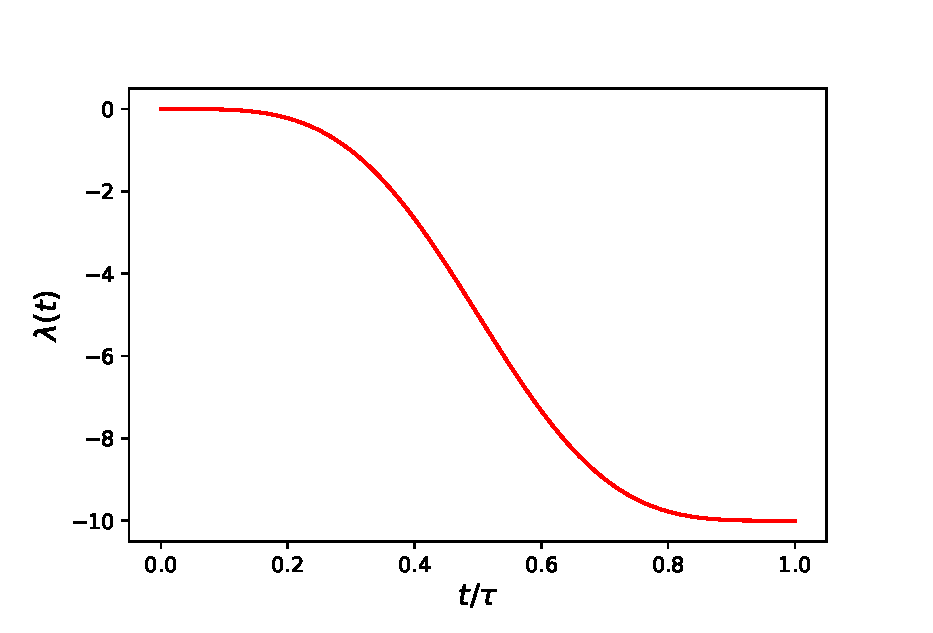
\includegraphics[scale=0.67]{protocol.eps}
\caption{Protocol chosen for going from $\lambda_i=0$ to $\lambda_f=-10J$ in time $\tau$}
\label{protocol_figure}
\end{figure}

The \textit{naive} way to drive our system will be take just our bare Hamiltonian $H_b$ and see the performance by computing $F^2$ and $E-E_0$ as we change duration of protocol $\tau$. This is shown in blue line of figure \ref{fid_energ}. We note that increasing $\tau$ improves our performance no matter how we drive our system because we are going towards adiabatic limit.


For our $\lambda$ - dependent  Hamiltonian $H_0$, approximate gauge potential is chosen to be 
\begin{equation}
A_{\lambda}^*= \sum_j \alpha_j \sigma_j^y
\end{equation}
where $\alpha_j$ are found using variational approach given in \cite{sels2017minimizing}. They find that $\alpha_j$ for $H_0$ is given by 
\begin{equation}
\alpha_j= \dfrac{1}{2} \dfrac{Z_j X_j^{\prime}- X_j Z_j^{\prime}}{Z_j^2 + X_j^2 +2J^2}
\end{equation}
Now for our $H_b$, $\alpha_j$ is given by 
\begin{equation}
\alpha_j= \delta_{j,0} \dfrac{1}{6 + (\lambda +0.8)^2}
\end{equation}
Hence, our  Hamiltonian with gauge potential term (CD term)  will be :


\begin{eqnarray}
H_{CD}&=&H_b + \dot{\lambda} A_{\lambda}^* \\
&=&H_b + \dot{\lambda} \alpha_0 \sigma_0^y 
\end{eqnarray}

In red line of figure \ref{fid_energ}, we do find that Hamiltonian with local CD term $H_{CD}$ does indeed give a better performance by increasing fidelity $F^2$ and decreasing energy above ground state $E-E_0$ for short protocol duration $\tau$. 
In Dries's paper \cite{sels2017minimizing}, they show  similar results in their figure 4, where they have used spin chain of $L=15$.



\begin{figure}
\centering
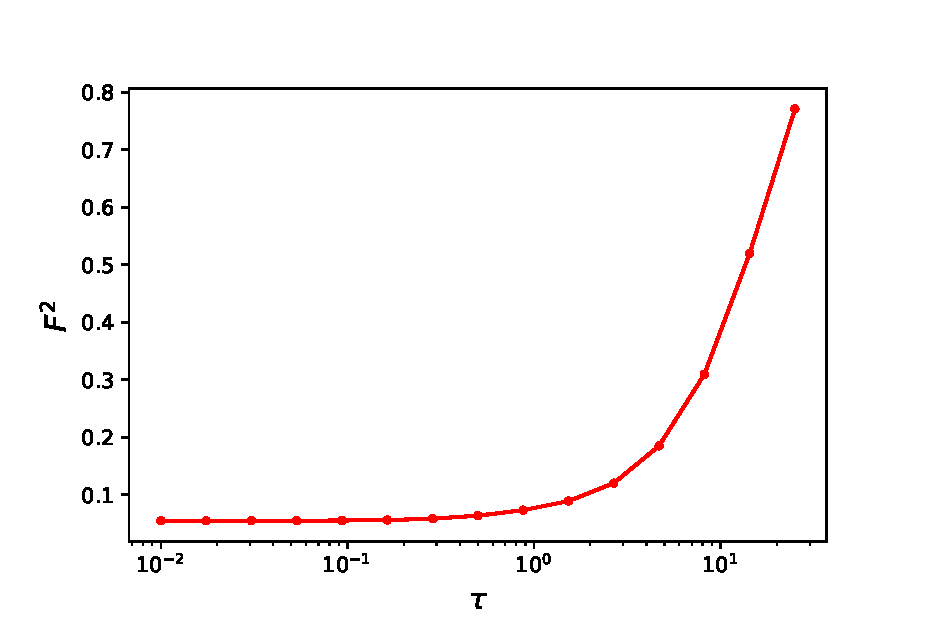
\includegraphics[scale=0.5]{fidelity_naive.eps}
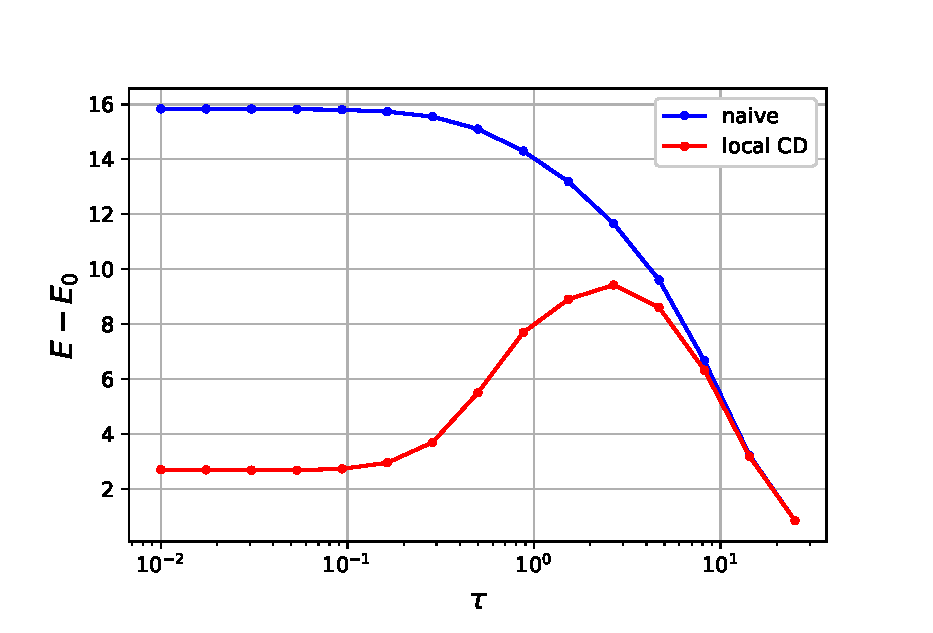
\includegraphics[scale=0.5]{final_energy_naive.eps}
\caption{Fidelity $F^2$ and final energy above ground state $E- E_0$ for L=12 spin chains}
\label{fid_energ}
\end{figure}

\section{Locality of operators: regulator}
We introduce a regulator/ cutoff $\mu$ to regularize our exact gauge potential for non-integrable chains:
\begin{eqnarray}
\langle n | A_{\lambda} | m \rangle &=& \lim_{\mu \rightarrow 0} \lim_{L \rightarrow \infty } i \hbar \dfrac{\langle n | \partial_{\lambda}H  | m \rangle}{(E_n-E_m)^2 + \mu^2} (E_n-E_m) 
\end{eqnarray}

Now we will use Laplace transform with $s= E_n-E_m$:

\begin{eqnarray}
\langle n | A_{\lambda} | m \rangle &=&  i \hbar \dfrac{\langle n | \partial_{\lambda}H  | m \rangle}{(E_n-E_m)^2 + \mu^2} (E_n-E_m) \\
&=& i \hbar  \int^{\infty}_{0} e^{-\mu t} \langle n | \partial_{\lambda}H  | m \rangle \sin((E_n-E_m)t) \\
&=& \dfrac{i \hbar}{2i}  \int^{\infty}_{0} e^{-\mu t} \langle n | \partial_{\lambda}H  | m \rangle \left( e^{i(E_n-E_m)t} - e^{-i(E_n-E_m)t} \right) \\
&=& \dfrac{ \hbar}{2}  \int^{\infty}_{0} e^{-\mu t}  \left(  \langle n | e^{iE_nt} \partial_{\lambda}H   e^{-i E_m t} | m \rangle  -  \langle n |e^{-i E_n t}  \partial_{\lambda}H  e^{ i E_mt} | m \rangle  \right) 
\end{eqnarray}
Hence, we can simplify our expression by defining propagator  $U= \exp(-i H t/ \hbar)$. We note that parameter $\lambda$ is fixed while we evolve it in the \textit{artificial time} $t$.
\begin{eqnarray}
A_{\lambda} &=& \dfrac{\hbar}{2 }\int_0^{\infty} e^{-\mu t} [U^{\dagger}(t \hbar) \partial_{\lambda} H U(t  \hbar) - U^{\dagger}(-t  \hbar) \partial_{\lambda}H U(-t \hbar)]  \\
&=& \dfrac{\hbar}{2 }\int_0^{\infty} e^{-\mu t} [ \partial_{\lambda} H (t \hbar) -  \partial_{\lambda}H (-t  \hbar)  ]  
\end{eqnarray}
where $\partial_{\lambda}H (t)$ is time-evolved operator $\partial_{\lambda}H$ in Heisenberg picture.

We would be using  Hadamard formula to simplify $\partial_{\lambda}H (t)$.

\begin{eqnarray}
\partial_{\lambda}H (t) &=& U^{\dagger}(t ) \partial_{\lambda} H U(t ) \\
&=& \exp(i H t/ \hbar) \partial_{\lambda} H \exp(-i H t/ \hbar)  \\
&=&  \partial_{\lambda} H  + \dfrac{i t}{ \hbar} [H, \partial_{\lambda} H] + \left(\dfrac{i t}{ \hbar}\right)^2 [H,[H, \partial_{\lambda} H]]  + \left(\dfrac{i t}{  3! \hbar}\right)^3 [H,[H,[H, \partial_{\lambda} H]]]   + \ldots
\end{eqnarray}
Similarly,  for $\partial_{\lambda}H (-t)$, we have:

\begin{eqnarray}
\partial_{\lambda}H (-t) &=&  \partial_{\lambda} H  - \dfrac{i t}{ \hbar} [H, \partial_{\lambda} H] + \left(\dfrac{i t}{ \hbar}\right)^2 [H,[H, \partial_{\lambda} H]]  - \left(\dfrac{i t}{  3! \hbar}\right)^3 [H,[H,[H, \partial_{\lambda} H]]]   + \ldots
\end{eqnarray}

Now we see that $\partial_{\lambda} H (t \hbar) -  \partial_{\lambda}H (-t  \hbar) $ contains only odd  power of time $t$:
\begin{eqnarray}
\partial_{\lambda} H (t \hbar) -  \partial_{\lambda}H (-t  \hbar)&=&  2 \left[ i t [H, \partial_{\lambda} H] + \left(\dfrac{i t}{  3! }\right)^3 [H,[H, \partial_{\lambda} H]]  + \left(\dfrac{i t}{  5! }\right)^5 [H,[H,[H,[H,[H, \partial_{\lambda} H]]]]]   + \ldots \right]  \nonumber \\
&=& 2 \sum_{n=0}^{\infty} \dfrac{(it) ^{2n+1}}{(2n+1)!} C^{2n+1} \\
%&=& -2 i \sum_{n=0}^{\infty} \dfrac{i^{2(n+1)} t ^{2n+1}}{(2n+1)!} C^{2n+1} \\
&=& 2 i \sum_{n=0}^{\infty} \dfrac{(-1)^{n} t ^{2n+1}}{(2n+1)!} C^{2n+1}
\end{eqnarray}
where $C^n$ is n- commutator of $H$ and $\partial_{\lambda} H$, i.e. $C_n= [H, [H, \mbox{ n times} \ldots,[H, \partial_{\lambda} H ]]] ] $

We can write short-hand notation for this $\sum_{n=0}^{\infty} \dfrac{(-1)^{n} t ^{2n+1}}{(2n+1)!} C^{2n+1}$ as $\sin ( C^{(1)}t)$, where $C^{(1)}= [H, \partial_{\lambda} H ]$. Thus, we can write: 
\begin{equation}
 A_{\lambda} =  i\hbar \int_0^{\infty} e^{-\mu t}  \sin ( [H, \partial_{\lambda} H ]t)
\end{equation}
I would emphasize that $A_{\lambda}$ depends on all odd powered commutators.


Another way which might be more useful is by writing it in series form and changing the order of integral and sum. If there is some singularity, then the order of summation and integration should be important. So, here is how we should write this:
\begin{eqnarray}
A_{\lambda} &=&  i\hbar \int_0^{\infty} e^{-\mu t} \sum_{n=0}^{\infty} \dfrac{(-1)^{n} t ^{2n+1}}{(2n+1)!} C^{2n+1} \\
 &=&  i\hbar  \sum_{n=0}^{\infty}(-1)^{n} C^{2n+1} \int_0^{\infty} e^{-\mu t}  \dfrac{ t ^{2n+1}}{(2n+1)!} \\
 &=&  i\hbar  \sum_{n=0}^{\infty}   (-1)^{n} \dfrac{ C^{2n+1}}{\mu^{2n+1}}
\end{eqnarray}

Now one thing which is good is that if we first take $\lim_{\mu \rightarrow 0}$, then $A_{\lambda}$ diverges. Thus, now divergence is more explicit. 

The correct limit is to take first $\lim L \rightarrow \infty$. If $C^n \propto L$ and $\mu \propto 1/L$, then our $A_{\lambda}$ would again diverge. Dammit!

\subsection{ Integrable model}

\subsubsection*{ZZ: doesn't grow at all}
\begin{equation}
H= J \sum_{j=1}^{L-1}  \sigma_j^z \sigma_{j+1}^z +  \lambda  \sigma_0^x
\label{zz}
\end{equation}


\begin{eqnarray}
[H, [H,[H, \partial_{\lambda} H]]] &=&  (16 J^2 + 8 \lambda^2) [H, \partial_{\lambda} H] = \alpha [H, \partial_{\lambda} H]\\
\end{eqnarray}

\begin{eqnarray}
[H, \partial_{\lambda} H] &=&  2 i J \sigma_0^y (\sigma_1^z + \sigma_{-1}^z) \\
\end{eqnarray}
 Hence, $C^{2n+1}= \alpha^n C^{(1)}$

$A_{\lambda} =  i\hbar  C^{(1)}\sum_{n=0}^{\infty}   (-1)^{n} \dfrac{ \alpha^{n}}{\mu^{2n+1}}
$ 

\subsubsection*{ZZ with X:  grow ``slowly"}


\subsection{Non-integrable model}

\appendix

\section{Spin 1/2 particle in a time-dependent magnetic field}
I would include a derivation from lecture notes to gain an intuition here. I also plan to understand Berry's paper and reproduce some of his calculations in this appendix.

\section{Free interacting fermions in an external potential}

\begin{equation}
H_0= -J \sum_{j=1}^{L-1} (c^{\dagger}_j c_{j+1} +c^{\dagger}_{j+1} c_{j}) + \sum_{j=1}^{L} V_j(\lambda) c^{\dagger}_jc_j
\end{equation}


\begin{equation}
\mathcal{A}^*_{\lambda}= i  \sum_{j=1}^{L-1} \alpha_j (c^{\dagger}_j c_{j+1} - c^{\dagger}_{j+1} c_{j}) 
\end{equation}

I should include pictures drawn using sympy here.


\section{Classical adiabatic gauge potential}
Let's start by considering classical systems. For such systems, we specify the system by defining Hamiltonian $H (\lambda)$ in terms of canonical variables $q_i (\lambda,t)$ and $p_j (\lambda,t)$. where $\lambda$ is an externally controlled parameter. These variables satisfy the canonical relations:
\begin{equation}
\{q_i,p_j \}=\delta_{ij} 
\end{equation}
where $\{\ldots \}$ denotes the Poisson bracket.

Canonical transformations are transformations of $q_i$ and $p_j$ to new variables $\bar{q_i}$ and $\bar{p_j}$ such that it preserves Poisson bracket. Hence, 
\begin{equation}
\{\bar{q_i},\bar{p_j} \}=\delta_{ij} 
\end{equation}

What are gauge potentials? Gauge potential $A_{\lambda}$  are the generators of continuous canonical transformations in parameter $\lambda$ space , which can be defined as :
\begin{alignat}{5}
q_j(\lambda + \delta \lambda) & =& q_j - \dfrac{\partial A_{\lambda}}{\partial p_j} \delta \lambda &\Rightarrow & \dfrac{\partial q_j}{\partial \lambda} &=& -\dfrac{\partial A_{\lambda}}{\partial p_j} = \{A_{\lambda},q_j \} \\
p_j(\lambda + \delta \lambda) & =& p_j + \dfrac{\partial A_{\lambda}}{\partial q_j} \delta \lambda & \Rightarrow & \dfrac{\partial p_j}{\partial \lambda} &=& \dfrac{\partial A_{\lambda}}{\partial q_j}=\{ A_{\lambda},p_j \}
\label{def_A}
\end{alignat}

We can verify that these transformations are canonical upto order $\delta \lambda ^2$ because we can show that:
\begin{equation}
\{q_j(\lambda + \delta \lambda), p_j(\lambda + \delta \lambda)\} = \delta_{ij} + O(\delta \lambda ^2)
\end{equation}

Let's try to understand by taking an example of continuous canonical transformation. We would shift the position coordinate by $X_i$. Here our parameter $\lambda$ is $X_i$
\begin{eqnarray}
 q_i(X_i,t) &=& q_i(0,t) - X_i \\
p_i(X_i,t)&=& p_i(0,t)
\end{eqnarray}
Using equation \ref{def_A}, we see that $\frac{\partial A_{X_i}}{\partial q_j}=0$ and $-\frac{\partial A_{X_i}}{\partial p_j}=-\delta_{ij}$. Hence, $A_{X_i}=p_j + C_j$, where $C_j$ are arbitrary constants of integration. This is the gauge choice we have got in defining these gauge potentials. 

\bibliography{ref} 

\bibliographystyle{plain}


\end{document}